% Intended LaTeX compiler: pdflatex
\documentclass[10pt,a4paper,UTF8]{article}
\usepackage{zclorg}
\author{emacsun}
\date{}
\title{Emacs Tweet}
\hypersetup{
 pdfauthor={emacsun},
 pdftitle={Emacs Tweet},
 pdfkeywords={},
 pdfsubject={},
 pdfcreator={Emacs 25.0.50.1 (Org mode 9.0.5)}, 
 pdflang={English}}
\begin{document}

\maketitle
\tableofcontents
\titlepic{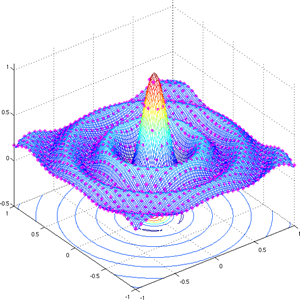
\includegraphics[scale=0.25]{../../img/sinc.PNG}}

\section{spacemacs中支持的text object.}
\label{sec:org7a107aa}

\begin{center}
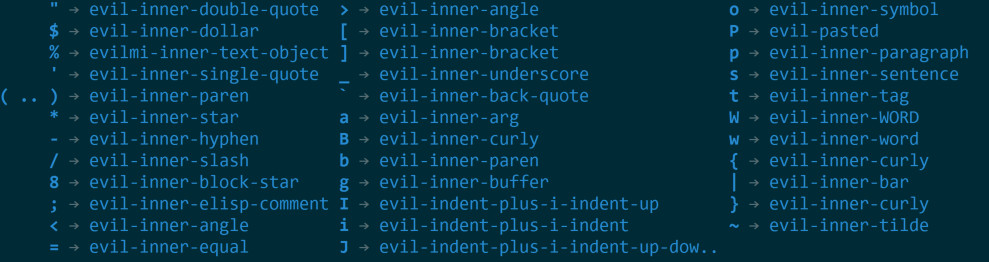
\includegraphics[width=0.6\textwidth]{../../img/20170217spacemacsTxtObject.jpg}
\label{org30fc8b8}
\end{center}

\section{spacemacs快捷键定义}
\label{sec:org04d19d9}
\textit{[2017-02-17 Fri 21:30]}
有几个快捷键失灵或者被覆盖,特意在 \texttt{.spacemacs} 中重定义。
\begin{center}
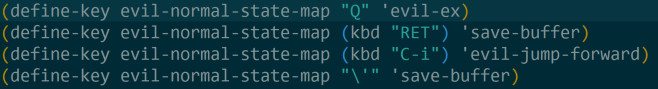
\includegraphics[width=0.6\textwidth]{../../img/20170217spacemacsSeveralShortkey.jpg}
\label{org545a52c}
\end{center}

在evil的normal模式中按下ENTER或者 \texttt{'} 键保存修改。这比 \texttt{:w} 或者 \texttt{SPC f s} 都方便。

\section{spacemacs 定义文件保存快捷键}
\label{sec:org3978c45}


\lstset{language=Lisp,label= ,caption= ,captionpos=b,numbers=none}
\begin{lstlisting}
(define-key evil-normal-state-map "\'" 'save-buffer)
(define-key evil-normal-state-map "’" 'save-buffer)
(define-key evil-normal-state-map "‘" 'save-buffer)
(define-key evil-normal-state-map (kbd "RET") 'save-buffer)
\end{lstlisting}

在normal模式中按下  '  \texttt{‘}  \texttt{’} 或者 \texttt{<RET>} (回车键)都可以实现文件保存的目的。

\section{spacemacs 循环切换item符号}
\label{sec:org43cfd44}


在spacemacs中,可以通过 \texttt{1.} 为多个项目或者步骤编号,比如 \texttt{1.} 代表第一步, \texttt{2.} 代表第二部,依次类推,如下所示:
\lstset{language=org,label= ,caption= ,captionpos=b,numbers=none}
\begin{lstlisting}
1. 第一步
2. 第二步
3. 第三步
\end{lstlisting}

当需要添加下一个步骤时,只需要在当前步骤按快捷键 \texttt{<ALT>-<RET>} 即同时按下 Alt和回车,即可添加下一步。

另一个小窍门是实用 \texttt{org-cycle-list-bullet} 命令来实现 item符号的改变。在spacemacs中绑定为 \texttt{-} 。 仍旧用上面的例子,当我们进入 \texttt{normal} 模式,把光标放到任意一个 \texttt{item} 的任意一个位置,按下 \texttt{-} 就会发现 \texttt{item} 符号发生了变化,比如我把光标放在“第二步” 的“二”字上,按下 \texttt{-} 就有
\lstset{language=org,label= ,caption= ,captionpos=b,numbers=none}
\begin{lstlisting}
A) 第一步
B) 第二步
C) 第三步
\end{lstlisting}

因为这个命令是 \texttt{cycle} 的,所以重复按下 \texttt{-} , \texttt{item} 符号会在Org支持的 \texttt{item} 符号之间切换。目前 Org支持的 \texttt{item} 符号有 \texttt{*} \texttt{+} \texttt{1.} \texttt{a)} \texttt{A)} .
\section{Emacs org 输出html中figure,table对齐}
\label{sec:org431920a}


在Emacs的org输出的html中,如果需要figure和table对齐,需在css中添加如下设置:
\lstset{language=css,label= ,caption= ,captionpos=b,numbers=none}
\begin{lstlisting}
div.figure{
    text-align:center;
}
table{
    text-align:center;
    margin-left:auto;
    margin-right:auto;
}
\end{lstlisting}
\section{JDEE 安装}
\label{sec:org9717c0e}


\begin{enumerate}
\item 在melpa中安装jdee
\item 安装jdee-server,(需要用到maven)
\item 
\end{enumerate}
设置 \texttt{JAVA\_HOME} 为 \texttt{C:\textbackslash{}Java\textbackslash{}jdk\_version\textbackslash{}} 而不是 \texttt{C:\textbackslash{}Java\textbackslash{}jdk\_version\textbackslash{}bin} 注意没有 \texttt{bin}
\section{使用Thinking in Java书中代码}
\label{sec:org4225876}


去 \href{http://www.mindviewinc.com/TIJ4/CodeInstructions.html}{这里} 下载代码,按照所示步骤添加 \texttt{CLASSPATH} 环境变量。由于TIJ侧重基础的学习,代码量都不是很大。因此学习TIJ, 只用Emacs JDEE即可完成所有操作。

在添加环境变量的时候一定要记得把 \texttt{.;..;} 也加入环境变量。
\section{定义复制整个buffer快捷键}
\label{sec:org7003904}
\textit{[2017-02-26 Sun 19:49]}
原来的快捷键为 \texttt{<SPC> b Y} ,太复杂还需要按下 \texttt{<SHIFT>} ,绑定后为 \texttt{<SPC> b y} 简单直接,拯救小拇指。
\lstset{language=emacs-list,label= ,caption= ,captionpos=b,numbers=none}
\begin{lstlisting}
(spacemacs/set-leader-keys "by" 'spacemacs/copy-whole-buffer-to-clipboard)
\end{lstlisting}
\section{Emacs Org中用到 | 时怎么办}
\label{sec:org7044205}
\textit{[2017-03-11 Sat 18:04] } 
Emacs Org的table使用 "|"来区分列,但是如果在表格中出现了条件概率\(P(A|B)\)这样的内容怎么办?答:使用转义字符 $\backslash$\(~\)vert
\section{Emacs Org 编辑代码快捷键}
\label{sec:org6c25f8b}


在Spacemacs Org中编辑代码段,使用 \texttt{C-c '} ,便会进入一个临时buffer,编辑结束后使用 \texttt{,c} 返回,使用 \texttt{,k} 放弃
\section{Emacs tab缩进配置}
\label{sec:org1b6dc8a}


目标:不插入tab字符,每次缩进四个空格。
\begin{verbatim}
(setq indent-tabs-mode nil)
(setq tab-width 4)
\end{verbatim}
\end{document}
